\chapter{Introduction}\label{ch:introduction}

Wind energy has emerged as one of the most promising technologies for the large-scale generation of electricity from renewable sources. The sustained growth in both size and number of wind turbines being installed globally has caused wind energy to outgrow its initial status as a fringe technology into a mature and cost-competitive component of the global energy landscape. Indeed, modern horizontal axis wind turbines are the largest rotating machinery ever built by mankind \citep{van2016long}, and wind energy has become a dominant power source in terms of installed capacity in the European Union, second only to natural gas, with capacity increasing from 13 GW to over 150 GW in the last 15 years (\citealp{windeurope}, see Figure~\ref{fig:windeurope}). In 2016, wind energy covered over 10\% of electricity demand in the European Union, and about 4\% worldwide \citep{gwec2017}. Given continuously decreasing costs, combined with targets for the renewable share in worldwide electricity generation portfolios \citep{EC,ren21}, global penetration of wind power is expected to further increase in the future. In spite of this progress, many interdisciplinary long-term research needs still remain in order to facilitate further rollout and cost reductions of wind power, for instance in the field of wind turbine materials, integration of intermittent and variable wind power in the electricity grid, and wind turbine control \citep{wind2013long,van2016long}.

\begin{figure}
	\centering
%	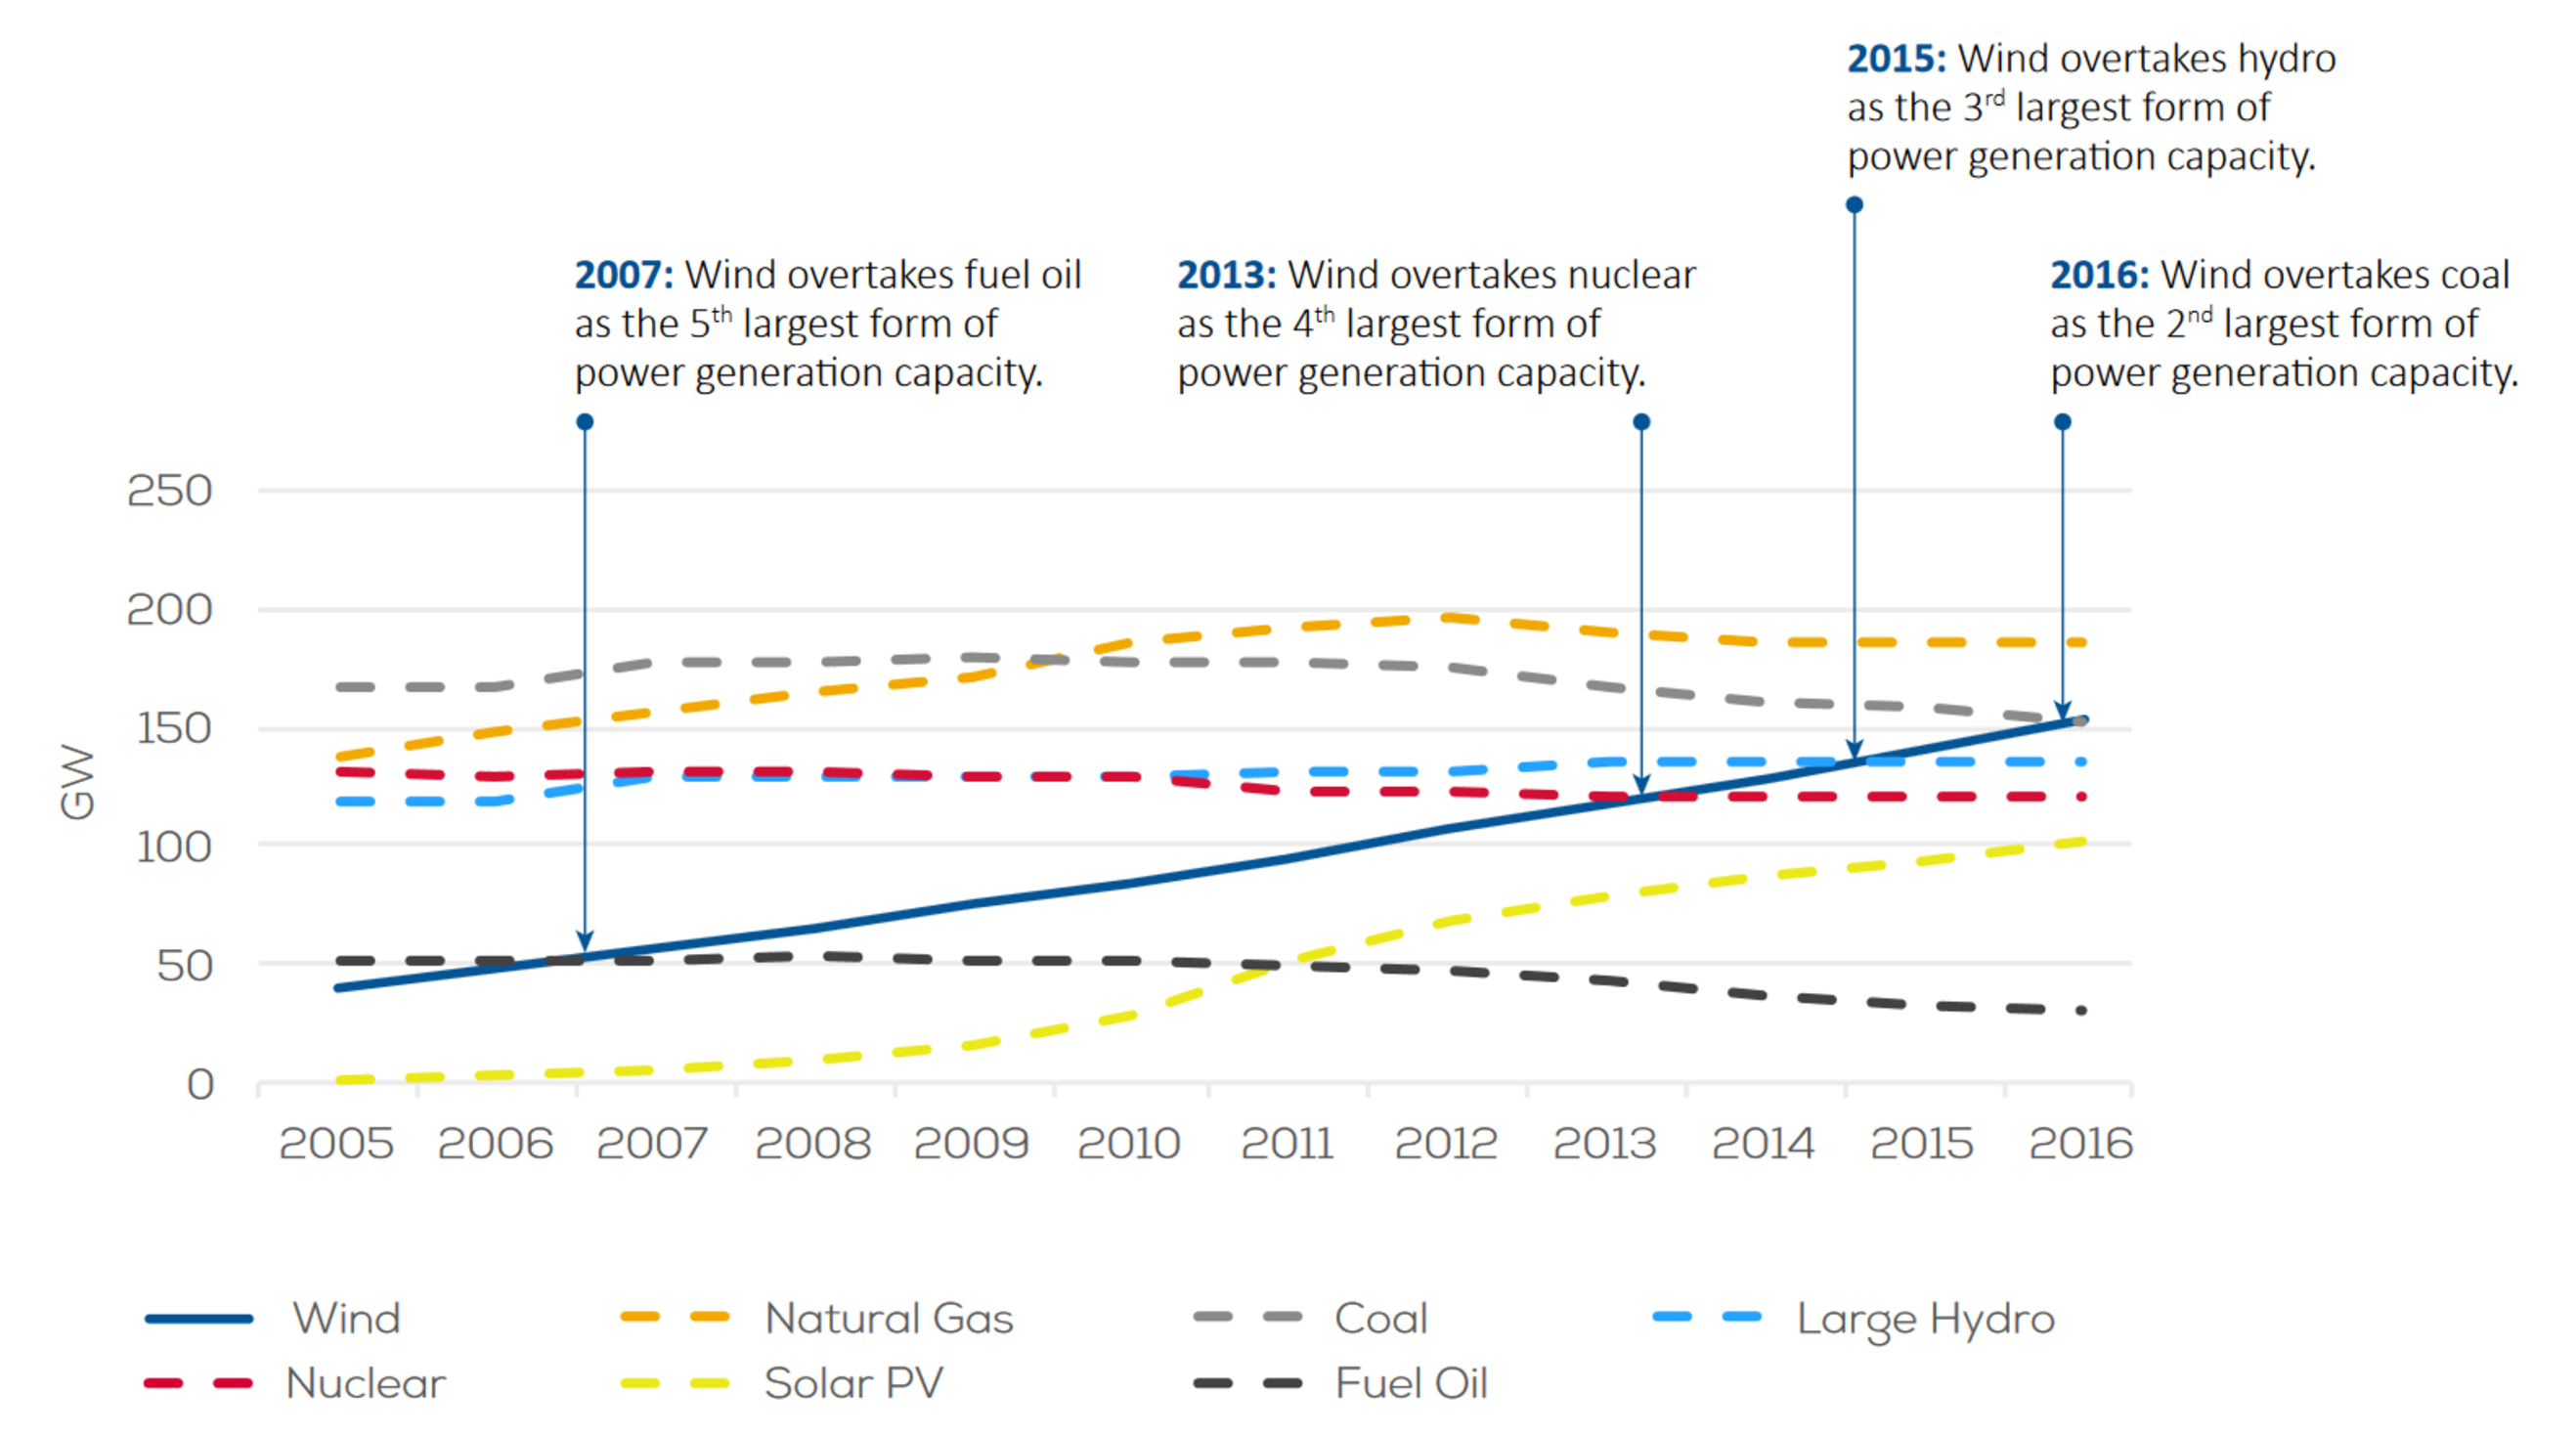
\includegraphics[width=\textwidth]{chapters/introduction/windeurope.eps}
	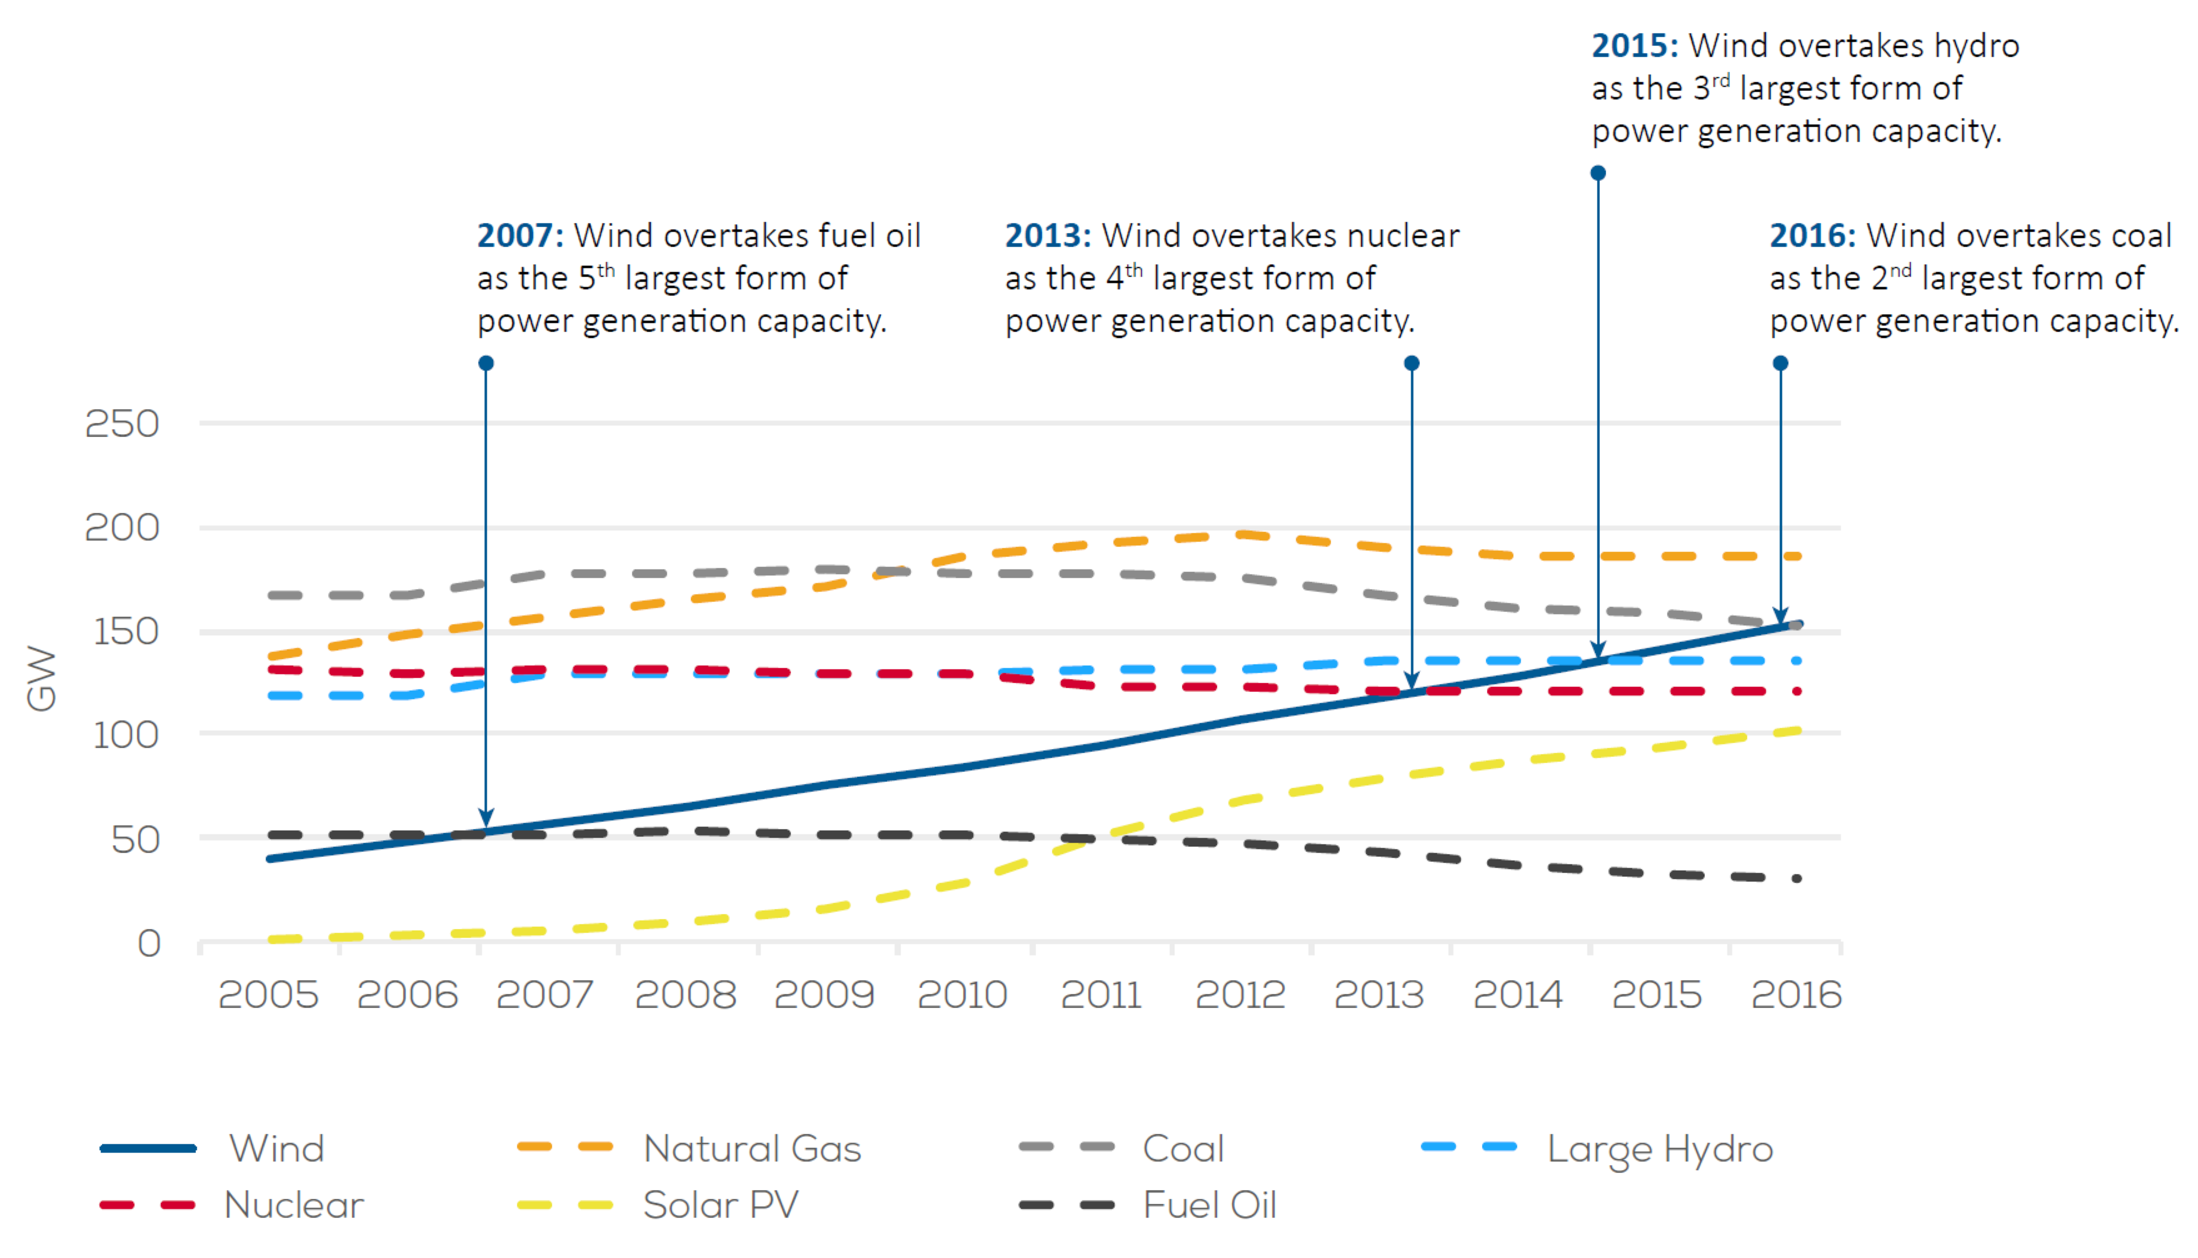
\includegraphics[width=\textwidth]{chapters/introduction/we3.eps}
	\caption{Cumulative installed power capacity by generation technology in the European Union 2005--2016. Reproduced from WindEurope, Wind in power: 2016 European statistics.  \label{fig:windeurope}}
\end{figure}

In practice, wind turbines are often sited together in wind farms. This is done because of economical reasons, e.g. due to easier maintenance and lower costs of land area and cabling. Furthermore, in case of bottom-mounted offshore wind turbines, the available area where the water is sufficiently shallow for mounting turbine foundations is often limited. In wind farms, complex aerodynamic interactions between neighboring wind turbines, as well as an interplay between the farm and the atmospheric boundary layer (ABL, i.e. the lower part of the atmosphere up to a few hundred meters, in which the wind is directly influenced by the ground surface) entail significant implications on downstream turbine behavior. More specifically, wake velocity deficits originating from upstream turbines and the associated increased turbulence in the flow field respectively, cause power deficits and increased dynamic loading in downstream turbines. For example, Figure~\ref{fig:horns_rev} illustrates the wind-farm flow field at the Horns Rev 2 wind farm off the western shore of Denmark. The figure illustrates the complex three-dimensional flow conditions imposed on the downstream turbines through the wakes of their upstream counterparts. Figure~\ref{fig:power_deficiency} illustrates the normalized power extraction for the Horns Rev 1 and Nysted wind farms. Depending on the wind direction, reductions in power extraction of up to 40\% are observed. Averaging over yearly wind conditions, this leads to wake-induced power losses in these farms in the order of 10\% (\citealt{jensen2005wake, barthelmie2010evaluation,barthelmie2010quantifying}). A similar decrease in the annual efficiency has been observed for many other wind farms, for instance Middelgrunden \citep{barthelmie2007modeling2}, Lillgrund \citep{dahlberg2009assessment} and Alpha Ventus \citep{westerhelweg2014wake},  with losses ranging between 5\% and 30\%.

In recent years, the prospect of mitigating these power losses through coordinated controllers at the wind farm level, instead of the individual turbine-level control applied today, has fueled a multitude of research investigations \citep{knudsen2015survey,boersma2017tutorial}. Continuing on preceding work by \cite{goit2015optimal}, the current thesis further investigates the application of optimal control techniques in large-eddy simulations of wind-farm boundary layers. In this approach, individual wind turbines are controlled dynamically by a supervisory wind-farm controller that puts them to use as flow actuators optimally influencing the ABL flow for enhanced farm power extraction. 

The current chapter is outlined as follows: Section~\ref{sec:intro_wfbl} firstly discusses wind-farm -- boundary layer interactions and introduces modeling tools for wind-farm flows. Section~\ref{sec:intro_les} further elaborates on the large-eddy simulation (LES) approach to wind-farm boundary layer simulations. Next, Section~\ref{sec:intro_control} discusses the current wind-turbine control paradigm applied to lone-standing turbines as well as turbines sited within a wind farm. Further, the state of the art and gaps in wind-farm control research are outlined. Thereafter, Section~\ref{sec:goitmeyersjfm} further discusses the prior work of \cite{goit2015optimal}. Subsequently, Section~\ref{sec:intro_aims} formulates the specific aims and objectives considered in this dissertation. Finally, Section~\ref{sec:intro_outline} provides the general outline of the current manuscript.

\begin{figure}[t]
	\centering
	
\includegraphics[width=0.9\textwidth]{chapters/introduction/HR2.eps}
	\caption{Horns Rev 2 wind farm with low-hanging fog visualizing wind turbine wakes. In the downstream regions of the farm, fog is dispersed by the additional wind-farm induced mixing with warm air aloft the array of turbines. Photo by: Bel Air Aviation -- Helicopter Services. Reproduced from Hasager et al. (2017) Wind farm wake: The 2016 Horns Rev photo case. Energies 10 (3). \label{fig:horns_rev}}
\end{figure}


\begin{figure}[t]
	\centering
	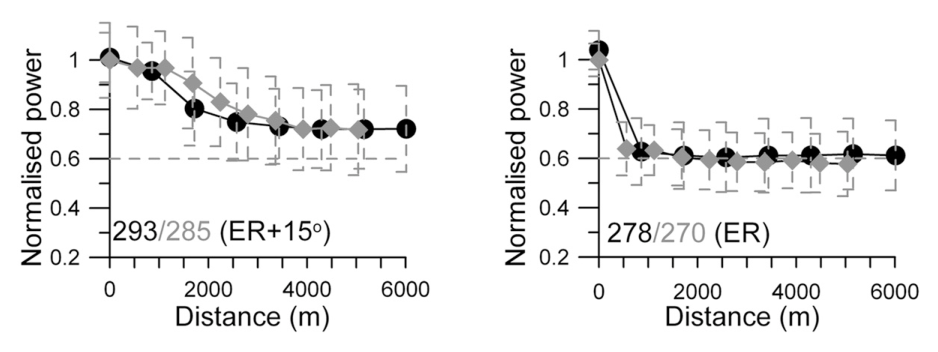
\includegraphics[width=0.9\textwidth]{chapters/introduction/power_barthelmie.eps}
	\caption{Normalized power extraction versus downstream distance for a wind direction with limited wake interaction (\emph{left}) and full wake interaction (\emph{right}). \textbf{Circles}: Nysted wind farm. {\color{gray} \textbf{Diamonds}}: Horns Rev 1 wind farm. Figure reproduced from Barthelmie et al. (2010) Quantifying the impact of wind turbine wakes on power output at offshore wind farms. J Atmos Ocean Tech 27 (8), 1302 -- 1317. \label{fig:power_deficiency}}
\end{figure}

\section{Wind-farm -- boundary layer interaction and modeling}\label{sec:intro_wfbl}
As illustrated by the discussion above, wind farms interact with the turbulent atmospheric boundary layer flow in several complex ways. By extracting energy from the boundary layer, the wind turbine leaves a wake signature in the flow, characterized by reduced wind speeds and increased turbulence. It was already mentioned that these wakes result in reduced power extraction and increased loading of downstream turbines. Furthermore, the behavior of wind-turbine wakes is strongly influenced by the characteristics of the atmospheric boundary-layer flow. 

Firstly, as the wake is advected downstream, its velocity deficit is attenuated through mixing induced by the turbulence in the ambient flow \citep{Chamorro2009}. Furthermore, the tendency to oscillate in the transversal direction upon propagating downstream, known as wake meandering, is triggered by specific turbulent structures in the ABL with lengthscales comparable to the rotor diameter \citep{espana2011spatial,espanawind}. Both the turbulent mixing and wake meandering partially alleviate adverse effects of the wake on downstream power extraction. 

Secondly, the thermal stability of the ABL greatly influences wake characteristics. During daytime, when surface heating results in a convective boundary layer, turbulence production through buoyancy increases overall mixing of the wakes, causing smaller velocity deficits in turbine wakes compared to neutral boundary layers, where turbulence production is dominated by shear \citep{zhang2013wind,abkar2015influence}. The opposite is true in nocturnal stable boundary layers that are characterized by long wakes with large velocity deficits and increase power losses \citep{barthelmie2010evaluation,dorenkamper}. Furthermore, also Coriolis forces influence wind-farm flows as the overall deceleration in downstream rows affects the horizontal force balance, resulting in a wind-direction change in downstream regions of large wind farms \citep{dorenkamper, allaerts2017boundary, van2017coriolis}.

%In the current work, a pressure-driven half-channel flow at very high Reynolds number is used as a surrogate for the neutral ABL flow. This implies that Coriolis and stability effects are not taken into account. Furthermore, the boundary-layer height is fixed at the top of the domain, instead of being characterized by capping inversion layer between the ABL and the free atmosphere above. The current approach relies on the assumption that wind turbines reside in the inner layer of the ABL, and has been widely applied in literature (see, e.g. \citealp{yang2012computational, porte2013numerical, nilsson2015large}).  It is believed that this approach is a good approximation for the purpose of benchmarking wind-farm control simulations in neutral ABLs of sufficient height (i.e. $\approx 10$ times turbine hub height). The implications of the current approach are discussed in further detail in \cite{calaf2010large}, \cite{goit2015optimal} Appendix B, \cite{allaerts2015large}, and \cite{allaerts2017boundary}. The remainder of this section focuses on modeling approaches for the wind-farm boundary layer interactions presented above.

\subsubsection{Wind-farm boundary layer modeling}
Turbulent wind-farm boundary layer flows are characterized by a large separation of scales. More specifically, wind-farm geometry and large atmospheric eddies are characterized by lengthscales in the order of kilometers whereas the dissipative Kolmogorov microscales reside in the millimeter range, thus the relevant lengthscales in wind-farm flows span over six orders of magnitude. This impedes direct numerical simulation (DNS) of these flows and has resulted in several modeling approaches, ranging from empirical and highly parametrized engineering models to Navier--Stokes based models that aim to resolve the most relevant flow physics. An extended survey of these approaches is provided in \cite{crespo1999survey} and \cite{sanderse2011review}. 

Building upon the seminal work of \cite{lissaman} in which the idea of superpositioning wakes from different turbines within a farm was introduced, several so-called wake models were developed. Notable models include the Jensen model \citep{katic1986simple, jensen1983note} and the FLORIS/FLORIDyn model \citep{gebraad2014data, gebraad2014control}. Although these models require careful parameter tuning and are unable to capture non-linear flow physics, they are cheap to evaluate and hence often used for control and design purposes. This explains their widespread use in both industry and control studies. A different approach is based on parabolized versions of the Reynolds-averaged Navier--Stokes equations \citep{ainslie88, crespo1988experimental, van2006improvements}. This allows to better capture non-linearities in the flow, but fails to resolve any unsteady turbulent flow features such as wake meandering or the passing of low-speed streaks, which are known to have a significant impact on wind-farm operation. Although the modeling tools in the current paragraph involve significant simplifications and cannot capture all relevant flow physics, their low computational efficiency merits the application in control and design studies, and explains the continuous further development of these methods by further parametrizing additional flow physics \citep{larsen2008wake, keck2014atmospheric, gebraad2016incorporating}. 

In recent years, the increase in computational power has facilitated the application of LES to wind-farm flows. In LES, the large energy-containing motions in the turbulent boundary layer flow are resolved with adequate spatio-temporal resolution, whereas the small-scale dissipative fluctuations are represented by a subgrid-scale model (see, e.g. \citealp{sagaut2006large}). This renders the technique particularly well suited for the simulation and physical understanding of wind-farm flows with minimal modeling assumptions: resolving energy-containing turbulent scales in the boundary layer allows the simulation of complex wind-farm behavior, such as unsteady fatigue loading, dynamic control, or variability due to changing atmospheric conditions. The application of LES to wind-farm flows is further discussed in the following section. 

\section{Wind-farm large-eddy simulations}\label{sec:intro_les}
As discussed above, LES is particularly well suited for the dynamic optimal control studies performed in this work. The current section provides a brief overview of LES applied to wind farms, and illustrates the challenge in generating turbulent inflow conditions for this application. A more detailed overview of the application of LES to wind turbines and wind farms can be found in \cite{sanderse2011review,mehta2014large} and, more recently, \cite{breton2017survey}. 

Although prior studies applied the LES technique to study the wake behind a single wind turbine \citep{troldborg2007actuator, jimenez2007advances, jimenez2008large}, the earliest adoption of the technique to a wind-farm flow can be found in \cite{ivanell2009numerical}. In the latter, two turbine columns of the Horns Rev 1 wind farm were simulated using periodic spanwise boundary conditions and synthetic turbulence inflow conditions derived from the Mann spectral model \citep{mann1998wind}. Comparisons with measurements were reasonable, although downstream turbines produced significantly less power than expected from measurement data.  \cite{calaf2010large} applied periodic boundary conditions on all horizontal domain boundaries, hence effectively simulating a fully-developed wind-farm boundary layer of infinite extent, and showed that power extraction in such `deep arrays' is governed by vertical transport of kinetic energy. Further examples on fully-developed wind farm LES include \cite{calaf2011large,yang2012computational,verhulst2014large,yang2014large,cortina2016distribution}; and \cite{sharma2017perturbations}. However, when entrance effects are to be simulated in actual wind farms, periodic boundary conditions cannot be invoked. Instead, unwaked turbulent inflow conditions have to be applied.

\subsubsection{Turbulent inflow conditions in wind-farm LES}
The generation of physically accurate turbulent inflow conditions containing coherent structures, physical phase relationships and non-Gaussian statistics is a long-standing issue in turbulence-resolving flow simulations. In the context of LES for wind energy, \cite{troldborg2007actuator} already pointed out the importance of adequate turbulent inflow conditions for accurate wake behavior and recovery. In recent years, the use of turbulent inflow conditions generated by so-called precursor methods has been increasing \citep{keating2004priori, tabor2010inlet} as an alternative to synthetic inflow methods as used in \cite{ivanell2009numerical}. In a precursor approach, a separate LES of a fully-developed boundary layer without wind turbines is run on an independent domain with periodic boundary conditions, from which data is extracted to be used as inflow conditions for a wind-farm LES. The use of Navier--Stokes based inflow turbulence is particularly attractive for wind energy applications since, in contrast to synthetic methods, this approach allows to capture the streaky turbulent structure of the neutral ABL, which can have an important influence on wake meandering and vertical entrainment of kinetic energy. \cite{churchfield2012large} used precursor inflow in a LES study of the Lillgrund wind farm. They attributed their better match to measurement data in comparison to \cite{ivanell2009numerical} to the fact that the synthetic inflow from the latter might not be able to properly trigger wake meandering. 
\cite{park2014large} applied a precursor-type approach to estimate turbine loading in a stable ABL. They strongly advocate the use of precursor methods because the assumptions invoked by synthetic methods may not uphold in atmospheric flows. \cite{stevens2014concurrent} developed a concurrent precursor method running in parallel to the main wind-farm simulation and applied this to a Horns Rev-like wind farm. Other examples of wind-farm LES with precursor-generated turbulence are \cite{porte2011large,archer2013quantifying,wu2013simulation,stevens2014large,abkar2016wake}; and \cite{stevens2016dependence}.

As further discussed in Chapter \ref{ch:turbulent_inflow}, it is widely accepted that precursor methods generate highly accurate turbulent inflow conditions \citep{keating2004priori,tabor2010inlet,wu2017inflow}. However, as indicated by \cite{esparza2014bridging} \emph{``$\dots$ they present problems when the flow direction changes, cannot be generalized for multiple inflow boundaries and are affected by contamination due to periodicity.''} This can present issues, e.g. when attempting to couple boundary-layer dynamics with large-scale temporal variations in the wind direction. 


%\section{Conventional Wind-farm control}
%Wind-turbine control (region I, II, III), degrees of freedom, main control paradigm.
%	
%\section{Coordinated wind-farm control}
%
%	\subsection{State of the art}
%	Current approach to wind-farm control studies
%
%	\subsection{Optimal wind-farm control}
%	Introduce Goit and Meyers, JFM
%
%	\subsection{Challenges}
%	Computational costs, infeasibility of optimal control in practice, generalization towards yaw and spatially-developing wind farms

\section{Turbine control in wind farms}\label{sec:intro_control}

The general aim of a wind turbine controller is to optimize power extraction from the wind while keeping structural and electrical loading of the turbine components at acceptable levels.

The kinetic energy flux through the rotor with area $A$ at a wind speed $V$ defines the total available power in the wind as $P_{\text{wind}} =(1/2)\rho A V^3$, with $\rho$ the air density. The aerodynamic performance of a wind turbine can then be quantified by means of a power coefficient, i.e. as the fraction of power in the wind that is captured by the turbine and converted to electricity in the generator as $C_P = P/P_{\text{wind}}$. It is well known in literature that the theoretical upper bound for $C_P$ in steady operation lies below unity at the so-called Betz limit, i.e. $C_P^{\text{Betz}} \approx 0.593$ (see, e.g., \citealp{burton2001wind,hansen2015aerodynamics}). This value results from a balance between extracting kinetic energy from the wind while maintaining a sufficient mass flow rate through the rotor. Modern wind turbines are able to achieve peak power coefficients of about 0.45 to 0.5 \citep{siemens6mw, vestas3mw}.

The remainder of this section discusses how the power coefficient can be influenced and details strategies for both isolated and clustered turbines. Firstly, the degrees of freedom in controlling a modern wind turbine are introduced and the conventional approach to turbine control is elaborated. Thereafter, the state of the art in wind-farm control is outlined. 

\subsection{Wind-turbine control}
Virtually all modern utility-scale turbines are variable-pitch variable-speed horizontal-axis wind turbines. The main parameters influencing the aerodynamics and power extraction characteristics in these wind turbines are the pitch angles of the blades $\beta$, the yaw angle of the rotor $\theta$, and the tip speed ratio $\lambda$, as illustrated in Figure~\ref{fig:WT_drawing}. The tip speed ratio is defined as the ratio between the rotor tangential speed at the rotor tip and the incoming wind speed $V$, i.e.  $\lambda = \Omega R /V$, with $\Omega$ and $R$ the rotational rate and radius of the rotor respectively. In practice, the rotational speed is governed by the balance between the resisting torque setpoint of the turbine generator $T_{\text{gen}}$ and the driving aerodynamic torque $T_{\text{aero}}$ enacted by the wind through the rotor blades, which in itself is a function of both $\lambda$ and $\beta$. The blade pitch angle and rotor yaw angle can be controlled directly through actuators mounted in the turbine hub. The remainder of this section briefly outlines the conventional wind-turbine control strategy employed in operational wind farms. A more elaborate overview of wind turbine control, including control loops, actuators and sensors can be found in \cite{pao2009tutorial}. 

In normal operation, the yaw system is used to turn the nacelle such that the rotor is perpendicular to the local wind direction. Figure~\ref{fig:WT_drawing}b,c illustrate the response surface of the power coefficient $C_P$ and thrust coefficient $C_T$ with respect to tip speed ratio and blade pitch angle for the NREL 5 MW turbine \citep{jonkman2009definition, annoni2016analysis}. The figure illustrates that maximal power extraction is attained for a single ($\lambda^*, \beta^*$) combination.

\begin{figure}[t]
	\centering
	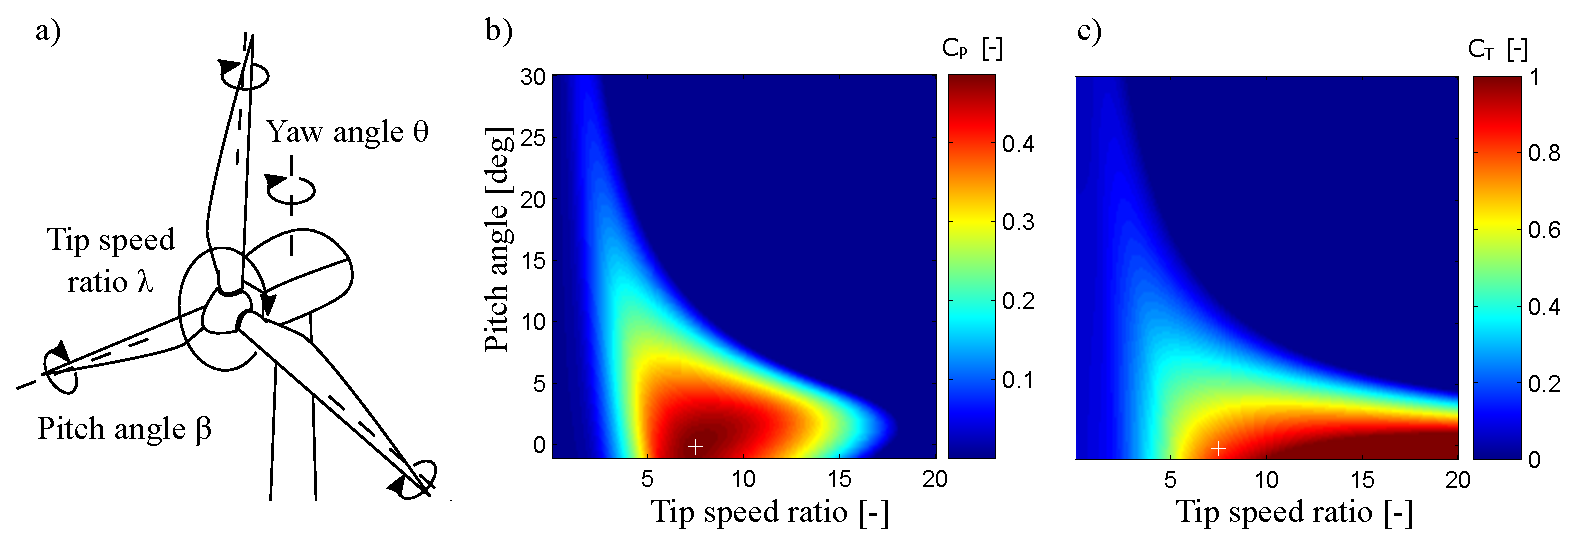
\includegraphics[width=\textwidth]{chapters/introduction/wt_drawing3.eps}
	\caption{\emph{a)} Parameters influencing wind-turbine aerodynamics. \emph{b-c)} Power coefficient $C_P$ and thrust coefficient $C_T$ as a function of tip speed ratio and blade pitch angle for the NREL 5MW wind turbine. The cross (+) indicates the maximum $C_P$ operation point. \emph{b)} and \emph{c)} reproduced from Annoni et al. (2016) Analysis of axial-induction-based wind plant control using an engineering and a high-order wind plant model. Wind Energy 19 (6), 1135 -- 1150. \label{fig:WT_drawing}}
\end{figure}

The conventional control paradigm to wind turbine control can be explained based on Figure~\ref{fig:regions}. Depending on the wind speed, three distinct regions are defined (see, e.g. \citealp{johnson2006control,laks2009control,pao2009tutorial}). When the wind speed is lower than the cutin wind speed $V_{\text{cutin}}$, the available power in the wind is insufficient to overcome losses in the energy conversion system and the wind turbine is not operated. This regime is defined as Region~1. With increasing wind speeds in Region 2, wind turbines are operated to extract as much power from the wind as possible, hence maximizing their power coefficients. In practice, this maximum is tracked by fixing the blade pitch at the optimal value $\beta^*$, while the optimal tip speed ratio $\lambda^*$ is attained by adapting the generator torque such that the rotor speed is tuned to the local wind speed. Upon further increase of the wind speed, this control strategy will bring the wind turbine to its rated conditions: nominal power $P_{\text{rated}}$ is extracted by turbine generator at the rated rotational speed of the rotor and rated wind speed $V_{\text{rated}}$ . From this point onwards, extracted power is kept constant to avoid overloading the generator and overspeeding the rotor. In practice, this is done by keeping the generator torque at a steady value while actuating the blade pitch to curtail power extraction, hence lower $C_P$. Finally, at very strong winds above the cutout wind speed $V_\text{cutout}$, the turbine is halted in order to protect it from excessive structural loading. 

\begin{figure}[t]
	\centering
	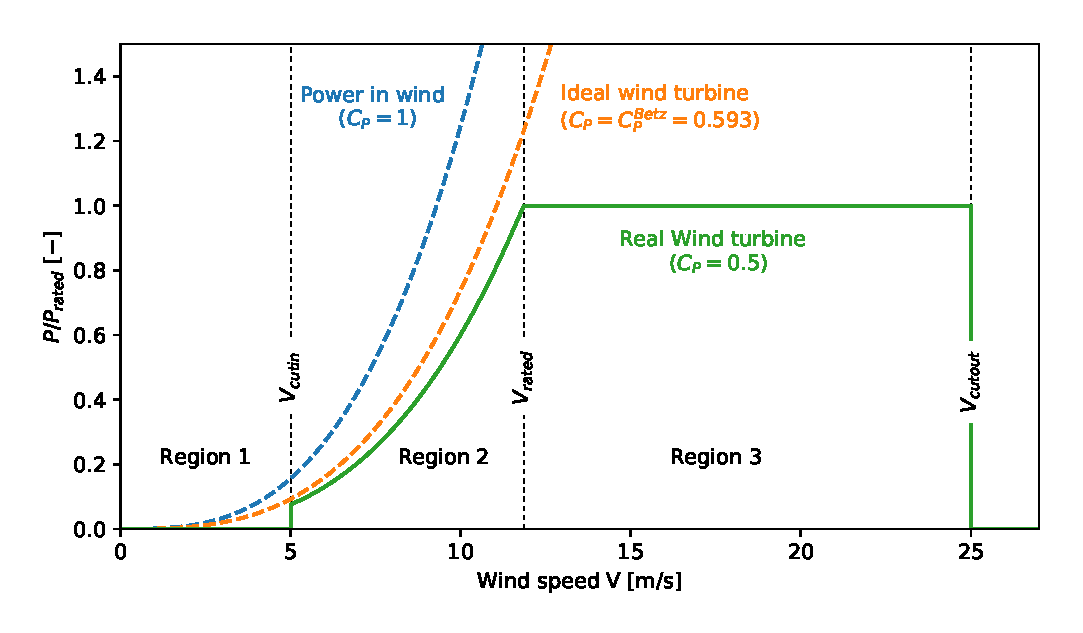
\includegraphics[width=\textwidth]{chapters/introduction/regions.eps}
	\caption{Steady-state power curve for a typical wind turbine. \label{fig:regions}}
\end{figure}

The current work focuses on wind speeds associated with Region 2 operation throughout the farm. From a wind-farm power maximization perspective, these speeds are relevant for coordinated wind-farm control since turbines operate below rated power, and more favorable local flow conditions directly translate into increased power extraction. It is important to note that Region 2 is in fact the most common operating regime in wind farms. For instance, the Horns Rev and Lillgrund sites are characterized by Region 2 wind speed over 80\% of the time \citep{bergstrom, Gryning2016}.
The Region 2 control strategy elaborated above is coined \emph{greedy} control throughout this text, as the turbine greedily optimizes its own power and loading behavior based on local flow conditions. Although this strategy works well for a lone-standing turbine, it does not take into account wake interactions for turbines in a wind farm or large-scale interplay between the ABL flow and the farm as a whole.  

%For higher wind speeds in Region 3, wind-farm power is capped by the rated powers of the turbines. If, in addition to power maximization, load mitigation is also considered, this operational regime also holds significant promise for coordinated control. The current thesis however focuses solely on power maximization. 



\subsection{Coordinated control in wind farms: state of the art}
The idea behind wind-farm control is to have a supervisory controller that optimizes overall wind-farm operation, based on aggregated information of the flow field and turbines within the farm, e.g. from measurements and/or some internal model. The objective of such a controller can be for instance maximizing wind-farm power extraction, following a total power reference signal, or minimizing fatigue loading of wind turbines within the farm. In contrast to the greedy control paradigm employed in current operational farms, a coordinated control approach allows to account for the interactions between turbines upon designing control laws. The promise of improving wind-farm performance through coordinated control has fueled a multitude of research efforts throughout the last decade. The remainder of this section provides an overview of some key studies on wind-farm control for power maximization. A more exhaustive survey of wind-farm control in a broader context can be found in \cite{knudsen2015survey} and \cite{boersma2017tutorial}.

The existing literature on wind-farm control for power maximization exhibits a dichotomy in control strategies between axial induction control and wake redirection control \citep{boersma2017tutorial}. Both strategies aim at improving the overall wind-farm efficiency by operating upstream turbines at locally non-optimal off-design conditions, altering the flow field through the wind farm such that power gains in downstream regions compensate for upstream efficiency losses. Furthermore, a distinction can be made based on the internal flow model used by the controller (ranging from model-free to control-oriented engineering models and LES) and the dynamics of the control law (i.e. static or dynamic control).

\subsubsection{Axial induction control}
The strategy behind axial induction control is to alter the induced slowdown of the incoming flow by deviating the tip speed ratio and/or blade pitch angle from their conventional setpoints $(\lambda^*, \beta^*)$, which directly translates to variations in power extraction and wake velocity deficit. As shown in Figure~\ref{fig:WT_drawing}b-c, in the vicinity of these conventional setpoints, the sensitivity of the power coefficient $C_P$ to setpoint variations is much smaller than that of the thrust coefficient $C_T$. This indicates that wake deficits can be reduced significantly with limited deviations in power extraction. The idea of axial induction control has been around for a long time as illustrated by the early study of \cite{steinbuch}, in which it was found that induction control could be used for increasing wind-farm power extraction. 

The conventional approach in designing a control law is to use tractable control-oriented engineering models, such as the Jensen wake propagation model \citep{jensen1983note, katic1986simple} introduced in Section~\ref{sec:intro_wfbl}. Alternatively, also a model-free approach can be used \citep{marden2013model, gebraad2015maximum, ciri2017model}. It is important that control strategies are tested in the presence of all relevant flow physics. Since actual wind-farm testing is both impractical and expensive, such testing was often omitted in early studies. Only in recent years, increased computational resources have facilitated testing in high-fidelity modeling environments such as the SOWFA LES platform \citep{churchfield2012large, fleming2013sowfa}. 

Studies on static axial induction control have attempted to increase overall power by statically curtailing upstream wind turbines \citep{knudsen2015survey}. Although some studies have indicated gains in the order of up to $5\%$ for selected cases (see, e.g., \citealp{horvat2012quasi, johnson2012assessment, gebraad2015maximum}), others have noted that gains predicted by engineering models were often not reproduced in high-fidelity environments \citep{annoni2016analysis}. \cite{nilsson2015large} performed an LES study of the Lillgrund wind farm, which is characterized by very strong wake interactions and power deficits, and is hence a prime candidate for axial induction control. However, simple static induction control failed to increase wind-farm power, indicating the need for more involved induction control strategies. In addition, recent wind tunnel studies have indicated discrepancies between power gains predicted by engineering models and those observed in the wind tunnel, and have reported no significant power gains beyond measurement uncertainties for static axial induction control  \citep{campagnolo2016wind, bartl2016experimental}. It is important to note that most of the studies on wind-farm control are performed in worst-case conditions, i.e. in which neighboring turbines are aligned with the mean wind direction, with maximal wake interaction and potential for coordinated control. Since wind farms are usually designed in such a way that these conditions occur rarely given the annual distribution of wind direction, the gains obtained by coordinated control should be high enough to have an effect on annual farm energy production. The viability of gains reported by many of the mentioned studies in actual wind-farm conditions is hence questionable.  

In a novel alternative approach, \cite{goit2015optimal} investigated \emph{dynamic} axial induction control by applying optimal control techniques directly in a high-fidelity LES model using adjoint-based methods. The wind turbines are used as dynamic flow devices acting upon the turbulent ABL flow without \emph{a priori} limiting the accuracy of the model flow physics representation. In this way, turbines are able to engage in active symbiosis with the physics governing the turbulent flow to increase overall power extraction, and energy extraction was increased by 16\% for the asymptotic limit of a fully-developed very large wind farm. This study is discussed in more detail in Section~\ref{sec:goitmeyersjfm} below.
\clearpage
\subsubsection{Wake redirection control}
Wake redirection control aims to steer wakes away from downstream turbines. In practice, this can be achieved either through individual pitch control, tilt control or through yaw control \citep{fleming2014evaluating}. Notwithstanding the fact that individual pitch control and, to a lesser extent, tilt control both show potential for increasing power and/or reducing loads \citep{bossanyi2003individual,fleming2015simulation,verhulst2015altering}, we will focus on wake redirection for power optimization through yaw control in the remainder of this discussion. Although nominally wind turbines are operated such that the rotor is perpendicular to the incoming flow, an intentional yaw misalignment can be used to induce transversal forces on the incoming flow. The opportunity to change inflow conditions for downstream turbines by redirecting wakes away from their rotors has incited a great amount of interest into characterizing the flow behavior of wind turbines in yaw and harnessing the associated deflection for wind-farm control. 

\cite{clayton1982measured} were the first to quantify the wake deflection behind turbines in yaw in an experimental study. Since then, numerous wind-tunnel investigations have further increased the understanding of the wake characteristics behind yawed turbines (see, e.g. \citealp{grant1997optical, medici2008measurements, bastankhah2016experimental}). \cite{jimenez2010application} performed an LES study to characterize wake deflection of turbines in yaw, and introduced an analytical model to quantify the displacement of the wake center. Recently, \cite{howland2016wake} combined numerical simulations with experimental measurements and found that counter-rotating vortices shed from the turbine rotor impose a curled shape on the deflected wake. 

\emph{Static} yaw control, in which upstream turbines intentionally misalign their rotors with incoming winds, has been proven as a promising approach to increasing power extraction, in numerical studies \citep{gebraad2016wind, quick2017optimization}, but also in wind-tunnel tests \citep{campagnolo2016wind2,park2017data} and full-scale field measurements \citep{soleimanzadeh2014state, fleming2017field}. Studies on \emph{dynamic} yaw control however are much more scarce. \cite{gebraad2015wind} applied a dynamic engineering model in order to incorporate time lag effects due to wake propagation. However, this model is unable to capture any turbulent mixing effects that have been shown to hold potential for enhanced wake recovery in the context of induction control as shown in \cite{goit2015optimal}. The possibility of unsteadily yawing turbines interacting with dynamic flow mechanisms has not been investigated to date. 

Furthermore, the combination of axial induction and wake redirection control has remained virtually unchartered terrain to date \citep{boersma2017tutorial}. Two notable exceptions on the combination of static induction and redirection control are the work of \cite{park2015cooperative} and \cite{park2017data}. \cite{park2015cooperative} investigated combined yaw--induction control using a steady-state engineering wake model. Results show significant promise, although the derived control strategies are not tested in a high-fidelity simulation environment. Recently, \cite{park2017data} applied a model-free data-driven approach for the control of both yaw and blade pitch angles for a small array of wind turbines in a wind tunnel. The control optimizer encouraged turbines to deviate yaw angle and, to a lesser extent, pitch angles from their greedy setpoints. However, no estimate was made on the surplus gains achieved by incorporating induction control in addition to yaw control only. 

\section{Optimal control in wind-farm boundary layers: preceding work of Goit \& Meyers (2015)}\label{sec:goitmeyersjfm}

\begin{figure}
	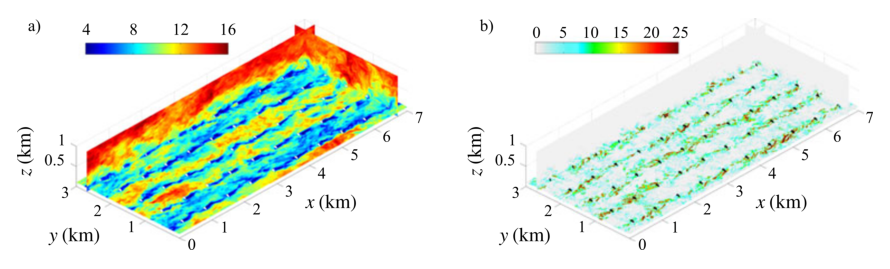
\includegraphics[width=\textwidth]{chapters/introduction/forward_adjoint4.eps}
	\caption{Flow field \emph{(a)} and adjoint flow field \emph{(b)} for a fully-developed `infinite' wind farm. Reproduced from Goit \& Meyers (2015) Optimal control of energy extraction in wind-farm boundary layers. J Fluid Mech 768, 5--50. \label{fig:flowfield_intro}}
\end{figure}

\begin{figure}
	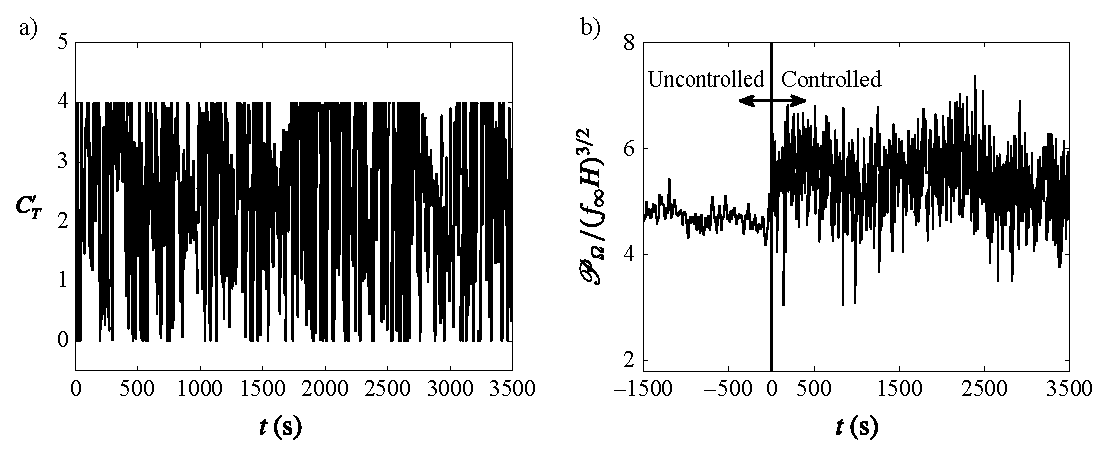
\includegraphics[width=\textwidth]{chapters/introduction/goit_meyers.eps}
	\caption{\emph{a)} Time evolution of the thrust coefficient $C_T'$ of one of the turbines in the optimally controlled farm. \emph{b)} Time evolution of wind-farm power extraction. Time $t = 0$ s indicates the moment when optimal control is activated. \label{fig:goitjfm} Reproduced from Goit \& Meyers (2015) Optimal control of energy extraction in wind-farm boundary layers. J Fluid Mech 768, 5--50. \label{fig:ct_power_goit}}
\end{figure}

In a novel approach to wind-farm control, \cite{goit2015optimal} applied optimal control directly in a wind-farm LES model using continuous adjoint-based methods in the pseudo-spectral SP--Wind framework. In this way, the turbines were used as dynamic flow devices acting upon the turbulent ABL flow without \emph{a priori} limiting the accuracy of the flow physics representation. Figure~\ref{fig:flowfield_intro} illustrates the flow field throughout the wind farm and the associated adjoint flow field. The latter is used to calculate the sensitivity of total wind-farm power to variations in control setpoints for the optimal control problem with partial differential equation (PDE) constraints in a tractable way, with a computational cost independent of the control space dimensionality. Further details and flow applications on the adjoint method can be found in \cite{giles2000introduction,bewley2001dns}; and \cite{troltzsch}. Since its introduction in a wind-farm control context by Goit and Meyers, the adjoint methodology has been applied in a control-oriented two-dimensional Navier--Stokes model \citep{boersma2016control,vali2016predictive}, a reference power tracking study with a one-dimensional wake model \citep{shapiro2017model}, and a layout optimization study using a steady-state Reynolds-averaged Navier--Stokes approach \citep{king2017optimization}.

In the study of Goit \& Meyers, the asymptotic limit of a fully-developed aligned wind farm of infinite size is considered. This limit has been shown to be relevant in the downstream regions of very large wind farms with a streamwise extent of at least tens of kilometers. Instead of resolving the effects of tip speed ratio and blade pitch angle on the induced thrust force as in Figure~\ref{fig:WT_drawing}c, they perform optimal axial induction control by dynamically controlling individual turbine thrust coefficients directly. An example of the time evolution of such a thrust coefficient for a given turbine is shown in Figure~\ref{fig:ct_power_goit}a. It can be seen that the turbine exhibits complex and highly unsteady behavior. By invoking and harnessing turbulent flow mechanisms responsible for wake mixing and kinetic energy transport, the optimally controlled wind turbines were able to increase power extraction by 16\% compared to a conventionally-controlled farm, as illustrated in Figure~\ref{fig:ct_power_goit}b. 

It is important to remark that, because of the large computational cost associated with the repeated PDE simulations throughout the optimization process, the methodology of Goit \& Meyers allows to benchmark control potential, but is not applicable as a real-time wind-farm controller. Instead, the idealized approach can provide valuable insight into the flow physics of optimally controlled wind farms, which could be used as a first step towards developing real-time controllers that approximate optimal control performance. However, coherent behavior linking simple dynamic control actions to an increase in power extraction was not identified in their study. 

Further, due to the assumption of a fully-developed wind-farm boundary layer, spatially developing features could not be resolved. However, as observed in Figure~\ref{fig:horns_rev}, turbines in the entrance region of actual wind farms are subjected to significantly different flow behavior than turbines in the far downstream regions. Furthermore, the strongly heterogeneous power extraction profile illustrated in Figure~\ref{fig:power_deficiency} indicates that entrance effects have a significant impact on overall wind-farm flow behavior. \cite{goit2016optimal} performed a first optimal control study of a spatially developing wind-farm boundary layer. However, due to the very large time-to-solution caused by the repeated PDE simulations, they considered only a single case with a limited amount of optimization iterations. 
%
%In order to simulate more cases for different setup parameters, it is important to reduce their computational time. To this end, a twofold approach can be followed: on one hand the \emph{amount of PDE simulations} for an optimization should be kept to a minimum, and on the other hand the \emph{computational cost per PDE simulation} should be reduced. In order to accomplish the first objective without reducing the gains achieved by the optimizer, a suitable optimization algorithm with most favorable convergence properties should be selected. Progress towards the second objective should come from harnessing parallelism on modern high-performance computing (HPC) systems, as the expected performance gains in code execution for future generation processors are limited \citep{sutter2005software}. 

Finally, it can be seen from Figure~\ref{fig:ct_power_goit}a that the straightforward application of optimal control techniques leads to fast variations in turbine setpoints. This behavior is undesirable for real turbines as it would require very fast control response and impose additional unsteady loading.

\section{Aims and objectives}\label{sec:intro_aims}
The main goal of this dissertation is to further explore dynamic optimal control of wind farms using the adjoint-based large-eddy simulation method introduced in \cite{goit2015optimal}, and obtain key insights into the flow physics of optimally controlled wind-farm boundary layers. This could serve as a first step towards the design of real-time wind-farm controllers that actively influence the boundary-layer flow for increased power extraction. In order to accomplish this, the SP--Wind optimization framework used by Goit \& Meyers should be significantly accelerated to perform control studies within a reasonable computational time. Further, the framework should be extended to allow the simulation of actual wind farms with entrance effects by imposing high-quality unsteady and coherent turbulent inlet conditions. 

This thesis also aims to investigate some of the remaining open issues left unanswered by previous control studies. The influence of the imposed smoothness of wind turbine dynamics on achievable power gains will be quantified. Further, expanding the control parameters from the axial induction study of Goit \& Meyers to also include yaw, this thesis investigates optimal wake redirection through unsteady yaw control, and explores the potential of combining dynamic induction control with dynamic yaw control. 

The main objectives can be formulated as follows: 
\begin{enumerate}
	\item Accelerate the in-house solver SP--Wind to be able to run more optimal control cases with better convergence in a shorter time to solution. More specifically, 
		\begin{itemize}
			\item Implement a  \emph{more scalable parallelization} algorithm for solving the forward and adjoint Navier-Stokes equations, thus leading to \emph{faster} functional and gradient evaluations for the optimization problem at hand.
			\item Upgrade the \emph{optimization algorithm} of the control framework to an algorithm with more favorable convergence properties than the classically used conjugate-gradient method, thus leading to \emph{fewer} functional and gradient evaluations for a given decrease in the cost functional.
		\end{itemize}
	\item Expand the capabilities of the SP--Wind framework to simulate spatially developing wind-farm boundary layers with entrance effects using high quality turbulent inlet conditions.  
		\begin{itemize}
			\item Implement a \emph{fringe region} technique to circumvent the inherent periodicity imposed by the pseudo-spectral numerics of the framework and allow non-cyclic boundary conditions. 
			\item Implement a \emph{precursor} method for generating unsteady and coherent turbulent inflow conditions. Further contribute to the development of precursor methods for general applications by generalizing them to multiple inflow directions, and deriving novel boundary conditions circumventing possible pollution of inflow data originating from the periodic boundary conditions in the precursor.
		\end{itemize}
	\item Further explore optimal dynamic induction control in spatially developing wind-farm flows. Assess the influence of temporal smoothness of wind turbine dynamics by including a finite wind-turbine response time to variations in control setpoints dictated by the optimizer. 
	\item Explore the potential of optimal yaw control and its combination with optimal induction control. Derive the novel required adjoint gradient and adjoint equations for yaw control.
	\item Analyze optimal control results with the aim of gaining insight into flow physics as a first step toward the development of practical wind-farm controllers.
\end{enumerate}

\section{Outline}\label{sec:intro_outline}
The outline of this thesis is structured as follows. First, Chapter~\ref{ch:methodology} introduces the overall methodology of wind-farm LES used throughout this work. The governing equations and high-order Fourier pseudo-spectral discretization schemes are introduced, and the wind turbine actuator disk model is elaborated. The fringe region technique for imposing non-cyclic boundary conditions is introduced (\emph{objective 2}), and the newly implemented pencil grid partitioning is elaborated and tested (\emph{objective 1}). 

Next, Chapter~\ref{ch:turbulent_inflow} discusses turbulent inflow conditions. An overall discussion on turbulent inflow conditions is presented based on a comparison between synthetic turbulence and precursor methods, and the classic precursor implementation in SP--Wind is elaborated. Further, a new generalization of precursor methods to variable inflow directions is presented, and a new shifted periodic boundary condition for precursor simulations is introduced (\emph{objective 2}).

Subsequently, Chapter~\ref{ch:opt_formulation} discusses the general optimization problem for optimal coordinated control of wind-farm boundary layers. The receding-horizon approach is introduced, and the mathematical formulation of the PDE-constrained optimization problem is defined. The adjoint gradient evaluation is detailed and verified. A quasi-Newton optimization algorithm is introduced from literature and its better convergence properties in comparison to the standard conjugate-gradient method is illustrated (\emph{objective 1}). 

Thereafter, Chapter~\ref{ch:opt_induction} further explores optimal induction control of spatially developing wind farms, and quantifies the influence of wind turbine response time on attainable gains for both overinductive and underinductive dynamic axial induction control. Energy gains and turbine dynamics are presented, and the wind-farm flow field statistics are discussed (\emph{objective 3}).

Chapter~\ref{ch:opt_analysis} performs an analysis of the complex thrust controls generated by the optimizations in Chapter~\ref{ch:opt_induction} and attempts to quantify the associated mechanisms for power increase. Further, it presents first steps towards harnessing these mechanisms for real-time control in first-row turbines (\emph{objective 5}).

Next, Chapter~\ref{ch:opt_yaw} investigates optimal yaw control and the potential of combined yaw and induction control. Wind-farm operation is optimized for both a turbulent boundary layer and a laminar uniform flow case. Analysis of dynamic yaw angles results in simplified yaw control strategies that approximate optimal control power extraction. (\emph{objective 4 \& 5}). 

Finally, Chapter~\ref{ch:conclusion} summarizes the key contributions from the current work, and formulates suggestions for future research. 


%%%%%%%%%%%%%%%%%%%%%%%%%%%%%%%%%%%%%%%%%%%%%%%%%%
% Keep the following \cleardoublepage at the end of this file, 
% otherwise \includeonly includes empty pages.
\cleardoublepage

% vim: tw=70 nocindent expandtab foldmethod=marker foldmarker={{{}{,}{}}}
